\documentclass[spanish]{article}
\usepackage[spanish]{babel} %esto es para que las ondas estn en espaol
\usepackage{url} % para la bibliografia
\usepackage{sectsty}
\usepackage{graphicx}
\usepackage{tikz}
\usepackage{verbatim}
\usetikzlibrary{calc}

\usepackage[utf8x]{inputenc}

\newcommand{\sectionline}{%
  \nointerlineskip \vspace{\baselineskip}%
  \hspace{\fill}\rule{0.5\linewidth}{.7pt}\hspace{\fill}%
  \par\nointerlineskip \vspace{\baselineskip}
}

%Para que los numeros de las secciones estn del lado izquierdo del margen
\makeatletter
\def\@seccntformat#1{\protect\makebox[0pt][r]{\csname
	the#1\endcsname\quad}}
\makeatother

\begin{document}

\title{Investigaci\'{o}n 1 \linebreak
CC3008 - Sistemas Operativos Avanzados } 
\author{Carlos López (08107) y Héctor Hurtarte (08119) \\ 
Universidad del Valle de Guatemala}   
\date{Septiembre del 2010}
\maketitle

\tableofcontents

\pagebreak
\begin{abstract}

Presentamos características y conceptos principales propios del sistema operativo Linux, el cual está basado en el estándar POSIX (\textit{Portable Operating System Interface for Unix}).

Las características y módulos desarrollados son, en su mayoría, referentes al kernel y no sujetas a alguna distribución en especial de Linux.
\end{abstract}

\section*{Introducción}
El mundo del software ha experimentado, de algunos años hacia el momento, un desarrollo considerable del software \textit{open source}, o código abierto. Uno de los proyectos que impulsó el desarrollo de este tipo de fue el \textbf{kernel} de Linux, del que hablaremos a continuación. Linux es un sistema operativo que, en la mayoría de distribuciones, se distribuye como software de c\'{o}digo abierto. Este sistema operativo es una versión de UNIX que ha ganado una gran popularidad en los últimos años. 

Este trabajo de investigación intenta presentar un análisis de distintos elementos involucrados en este sistema operativo, como aplicación de los conocimientos adquiridos durante dos cursos de sistemas operativos. La investigación desarrollará temas como manejo de memoria, manejo de procesos, sistema de archivos, modificaciones al \textit{kernel}, etc. Los contenidos de este trabajo pretenden ser compartidos como parte de una serie de presentaciones sobre distintos sistemas operativos, de forma que se pueda comparar el acercamiento que cada uno le da a elementos comunes como los mencionados anteriormente.

%%% GENERALIDADES DE DISEÑO
\section{Generalidades de diseño}
Linux es un sistema \textbf{multiusuario} y \textbf{multitarea} con herramientas compatibles con UNIX. Su sistema de archivos respeta la semántica UNIX tradicional (Filesystem Hierarchy Standard \cite{FHSWikipedia}).

A medida que las PCs se volvieron más potentes y las memorias y discos más baratos, el \textit{kernel} minimialista de Linux se expandió para implementar más funcionalidades de UNIX. Aunque \textbf{velocidad} y \textbf{eficiencia} siguen siendo objetivos de diseño, mucho del trabajo actual en Linux se concentra en un tercer objetivo: \textbf{estandarización}. 

\paragraph{Estandarización} Uno de estos mecanismos de estandarización es POSIX, que define un conjunto de especificaciones de diferentes comprotamientos del sistema operativo. Linux-FT fue la primera distribución de Linux en certificarse según POSIX.1. Existe actualmente un el proyecto \textbf{Linux Standard Base} (LSB)\cite{LSBWikipedia} que intenta estandarizar varias distribuciones de linux en aspectos como la jerarquía del sistema de archivos, bibliotecas est\'{a}ndar, el \textit{X Window System}, etc. Sin embargo, este proyecto ha sufrido críticas en temas como el uso de paquetes \textbf{RPM} en contraste con los \textbf{deb} utilizados por Debian, y la pobreza de sus pruebas de conformidad.

A pesar de que muchas certificaciones de Linux contra estándares UNIX son difíciles de alcanzar (por tiempo y costo económico), soportar una amplia base de aplicaciones es importante para cualquier sistema operativo. Por tanto, la implementación de estándares es un objetivo de importancia en el desarrollo de Linux, aún si la implementación no es certificada formalmente. Además de el estándar básico de POSIX, Linux actualmente soporta la extención de \textbf{threads} y un subconjunto de las extenciones para \textbf{control de procesamiento en tiempo real}.

\subsection{Componentes de un sistema Linux}
Un sistema Linux está compuesto de tres secciones principales de código, según las implementaciones tradicionales de UNIX:
\begin{itemize}
	\item \textbf{Kernel}: Responsable de mantener las abstracciones importantes del sistema operativo, incluyendo elementos como la memoria virtual y los procesos:
	\begin{itemize}
		\item Provee funcionalidad para \textbf{ejecución de procesos}.
		\item Provee servicios para brindar acceso protegido y arbitrario a recursos del hardware.
	\end{itemize}
	\item \textbf{Bibliotecas del sistema}: Definen un conjunto estándar de funciones para que las aplicaciones interactúen con el \textit{kernel}. Implementan parte de la funcionalidad del S.O. que no necesita privilegios del código \textit{kernel}. La interacción con el \textit{kernel} (\textit{system calls}) involucra transferir el control de modo usuario a modo \textit{kernel} además de manejar los argumentos de las llamadas al sistema de la forma necesaria. Adem\'{a}s pueden proporcionar versionas m\'{a}s complejas de las llamadas al sistema (gesti\'{o}n de archivos con \textit{buffer} de C implementadas en bibliotecas del sistema), o incluso funciones que no se corresponden con ninguna llamada al sistema (algoritmos de ordenaci\'{o}n o funciones matem\'{a}ticas). 
	\item \textbf{Utilidades del sistema}: Son programas que realizan tareas individuales y especializadas. Pueden ser invocadas para configurar aspectos del sistema, otros pueden ejecutarse permanentemente (demonios), etc. 
\end{itemize}
\begin{center}
\includegraphics[width=9.5cm]{img/components.png}
\end{center}
\paragraph{Modo kernel}De la imagen anterior, lo más importante es notar la diferencia entre el \textit{kernel} y todo lo demás. Todo el código del \textit{kernel} se ejecuta en modo privilegiado del procesador con acceso a todos los recursos físicos: el \textbf{modo kernel}. Todo código de soporte al sistema operativo que no necesita ejecutarse en modo kernel se coloca dentro de las \textbf{librerias de sistema}.

El \textit{kernel} de Linux ha mantenido históricamente un diseño \textbf{binario monolítico}, una arquitectura donde el sistema operativo completo trabaja en espacio de \textit{kernel} (en contraste con otros S.O. modernos que adoptan mensajería para sus \textit{kernels}). La razón principal de un diseño monolítico es el \textit{performance}: Dado que todo el código y estrucutas del \textit{kernel} están en un mismo espacio de memoria, no se necesitan \textit{context switches} cuando un proceso llama a una función del S.O. o cuando se genera una interrupci\'{o}n de harware.


%%% CARACTERÍSTICAS
\section{Características}

Las siguientes caracter\'{i}sticas no est\'{a}n sujetas a una distribuci\'{o}n específica.

\subsection{Caracteristicas desde Perspectiva de usuario:}
\begin{itemize}
\item Multi-tarea: varios programas pueden correr al \textit{mismo tiempo}
\item Multi-usuario: varios usuarios pueden tener la sesión iniciada al mismo tiempo.
\item Multi-plataforma: corre en diferentes procesadores, no sólo Intel.
\item Multi-procesador: soporte de multi-procesamiento simétrico en las plataformas Intel y SPARC (dos diferentes procesadores compartiendo la misma memoria))
\item Multi-hilo: soporte para múltiples hilos de control en un cada uno de los espacios de memoria de un proceso.
\end{itemize}

\subsection{Caracter\'{i}sticas desde la perspectiva de un desarrollador u otros:}
\begin{itemize}
\item Protección de memoria entre procesos
\item Memoria virtual usando pagineo a disco: pagineo a una partición u otro sistema de archivos, con la posibilidad de añadir más espacio de $swapping$ en tiempo de corrida.
\item Piscina de memoria unificada: para programas de usuario y cache de disco (para poder aprovechar la memoria libre para cache o reducir el cache cuando se están corriendo programas $grandes$.
\item Librer\'{i}as ligadas dinámicamente compartidas (DLL's) y librerías estáticas, generalmente de GNU.
\item Compatible con POSIX a nivel de código fuente.
\item Soporte para diferentes sistemas de archivos.
\item Manejador de LAN (con SMB)
\item Diferentes protocolos de red
\end{itemize}

%%% HISTORIA
\section{Historia}
\paragraph{} El sistema operativo Linux inició su desarrollo en 1991 a manos del estudiante finlandés Linus Torvalds, que escribió y nombró Linux a un pequeño \textit{kernel} para el procesador 80386. Luego, lo puso a disposición general compartiendolo a través de internet, por lo que el \textit{kernel} representa un caso de desarrollo colaborativo por parte de usuarios en todo el mundo \footnote{El \textit{kernel} es el componente central de la mayoría de sistemas operativos; es un puente entre las aplicaciones y el procesamiento actual de los datos a nivel de hardware. Las responsabilidades del kernel incluyen el manejo de los recursos del sistema (comunicación \textit{hardware} - \textit{software}).}.

Es necesario hacer la distinción entre el \textit{kernel} de Linux y un sistema Linux completo. El primero es un software completamente original desarrollado desde cero, mientras que el segundo cuenta con multitud de componentes, algunos desarrollados a partir de cero para el sistema operativo y otros tomados de otros proyectos o desarrollados junto con otros equipos de desarrollo. 

El primer \textit{kernel} de Linux presentado al público fué la \textbf{versión 0.01} el 14 de mayo de 1991:
\begin{itemize}
	\item Solo se ejecutaba sobre procesadores Intel compatibles con el 80386 y hardware PC; y tenía limitado soporte para controladores de dispositivos.
	\item Aunque el subsistema de memoria virtual era básico, incluía soporte para utilización de páginas compartidas con un mecanismo de copia durante la escritura.
	\item Único sistema de archivos: Minix\footnote{Sistema operativo clone de UNIX desarrollado por A. Tanembaum para el curso de Desarrollo de sistemas operativos en la  Vrije Universiteit de Ámsterdam.\cite{MinixWikipedia}}. Esto cambió en la siguiente versión.
	\item Este \textit{kernel} sí implementaba adecuadamente los procesos UNIX con espacios de direcciones protegidos. 
\end{itemize}
Con fines de importancia, la siguiente versión relevante fue el \textit{kernel} de Linux \textbf{versión 1.0} lanzada en 1994. En esta versión:
\begin{itemize}
	\item Se incluyó conexi\'{o}n por red: soporte para protocolos est\'{a}ndar TPC/IP de UNIX y una interfaz \textit{socket} compatible con BSD, además de soporte de controladores para dipositivos IP sobre una red Ethernet.
	\item Permitía paginación sobre archvios de intercambio (swap) \cite{ArchivoAlegsa} y mapeo a memoria de archivos arbitrarios (solo lectura).
	\item Se proporcionó también emulación de coma flotante para procesadores que no tenían coprocesador matemático (includio en 80387).
	\item Se incluyó \textbf{comunicación interprocesos} (IPC) estilo UNIX System V: memoria compartida, semáforos y colas de mensajes. 
\end{itemize}
En este punto inició el desarrollo de la versión 1.1, pero dada la gran cantidad de parches para errores en esta versión, se adoptó el patrón estándar de numeración para versiones del \textit{kernel}: las versiones impares eran \textit{kernels} de desarrollo; los números pares hacían referencia a \textit{kernel} de producción. Esta práctica ya no es seguida, pero se mantuvo por algún tiempo.

La \textbf{versión 1.2} no ofrecía tantas mejoras de funcionalidad como la versión 1.0, pero soportaba mayor variedad de dispositivios (ahora incluyendo PCI). Además se incluyo soporte para modo 8086 virtual de la CPU 80386 para poder emular DOS. Esta distribución incluía soporte parcialmente implementado para SPARC, Alpha y MIPS. 

Luego de esta versión, se incorporaron una gran cantidad de funcionalidades nuevas que vieron la luz con la \textbf{versión 2.0}, lanzada en junio de 1996. Las dos características que dieron paso a un cambio en el número principal de la versión fueron:
\begin{itemize}
	\item Soporte para múltiples arquitecturas, incluyendo una versión alpha para 64 bits.
	\item Soporte para arquitecturas multiprocesador. 
\end{itemize}
Además, se incluyeron nuevas funcionalidades:
\begin{itemize}
	\item Se mejoró la gestión de memoria a fin de proporcionar \textit{caché} unificada para datos del sistema de archivos independientemente del mecanismo de \textit{caché} de los dispositivos de bloque. Esto generó mayor eficiencia en el uso de memoria virtual y sistema de archivos.
	\item El mecanismo de \textit{caché} del \textit{filesystem} se extendió a sistemas de archivos en red y se añadió soporte para archivos mapeados en memoria en modo de escritura. 
	\item Se mejoró el \textit{performance} de las comunicaciones TCP/IP y se incluyeron nuevos protocolos de red (AppleTalk, desarrollado por Mac y actualmente en desuso, y AX.25, para uso de radio-operadores, entre otros).
	\item Se añadió capacidad de montar software de red remoto y volúmenes SMB (Microsoft)\footnote{Protocolo de red que permite compartir archivos e impresoras (entre otros) entre nodos de una red. Utilizado principalmente por Microsoft Windows y DOS, aunque existe implementación libre: Samba.}. 
	\item Se incluyeron \textit{threads} internas del \textit{kernel} para gestionar dependencias entre módulos.
\end{itemize}
Las mejoras continuaron con el lanzamiento de la \textbf{versión 2.2} en enero de 1999:
\begin{itemize}
	\item Se añadió una versión para sistemas UltraSPARC.
	\item En las características de red se incluyó un sistema \textit{firewall} más flexible, unos mejores mecanismos de gestión de tráfico y soporte para ventanas de transmisión TCP\footnote{El tamaño de la ventana de recepción TCP es la cantidad de datos recibidos (en bytes) que pueden ser metidos en el buffer de recepción durante la conexión. La entidad emisora puede enviar una cantidad determinada de datos pero antes debe esperar un asentimiento con la actualización del tamaño de ventana por parte del receptor\cite{TCPWikipedia}.}.
	\item Se mejoró el sistema de archivos NFS (Network File System, nivel de aplicación OSI para sistemas distribuídos) añadiendo un demonio NFS en modo \textit{kernel}.
	\item Se rediseñaron los mecanismos de bolqueo para tratamiento de señales, interrupciones y algunas interrupciones I/O utilizando granularidad más fina con el fin de mejorar la velocidad de multiprocesamiento simétrico (SMP)\footnote{SMP involucra una arquitectura multiprocesador donde dos o más procesadores idénticos son conectados a una memoria principal compartida y son controlados por un solo sistema operativo\cite{SMPWikipedia}.}. 
\end{itemize}
Las \textbf{versiones 2.4 y 2.6} incluyen mayor soporte para SMP, mejoras en el sistema de gestión de memoria y un planificador de procesos con un algoritmo de planificación con complejidad \textit{O}(1), que además permite desalojar un proceso mientras se está ejecutando en modo \textit{kernel}.
En concreto la \textbf{versión 2.6} \cite{Linux2.6Kniggit}:
\begin{itemize}
	\item Inició el soporte para dispositivos incrustados (sin unidad de manejo de memoria), a través de la inclusión del proyecto $\mu$CLinux (iPodLinux).
	\item En el sentido contrario, ofrece soporte para arquitecturas \textit{Non-uniform memory access} (NUMA), en donde la memoria se accede en posiciones relativas a otro procesador o memoria compartida entre procesadores. Surge como un adelanto a SMP.
	\item También se incluye soporte para \textit{hyperthreading}, que permite a un solo procesador enmascarar a nivel de hardware dos o más procesadores, lo que permite aumentar el \textit{performance} en algunas circunstancias, aunque añade complejidad en la calendarización.admin
\end{itemize}
	
	

%%% MANEJO DE PROCESOS
\section{Manejo de procesos}

Linux usa un modelo de procesos similar a sistemas operativos basados en UNIX, basado en el est\'{a}ndar POSIX. 

\subsection{El modelo de \textit{fork()} y \textit{exec()}}

El est\'{a}ndar POSIX tiene como principios separar dos operaciones sobre los procesos: \cite[p. 748, cap.21]{sistosEN}
\begin{itemize}
	\item Creaci\'{o}n, creado con la llamada \textit{fork()}
	\item Ejecuci\'{o}n, creado con la llamada \textit{exec()}.
\end{itemize}

Ninguna de las dos operaciones son dependientes una de otra, es decir, un proceso puede ser creado sin ser ejecutado, simplemente continuar\'{i}a ejecutando el proceso padre. Tampoco es necesario crear un proceso para poder ejecutar uno: cualquier proceso puede llamar a $exec()$ y el proceso que actualmente estar\'{i}a ejecutandose se deja de ejecutar y el nuevo proceso empieza a ejecutarse en el contexto de el proceso existente.

En UNIX, un proceso abarca toda la informac\'{o}n que el sistema operativo necesita para seguir el contexto de la ejecuci\'{o}n de un proceso.

\paragraph{Identidad de un proceso}
La identidad de un proceso consiste en:
\begin{itemize}
	\item \textbf{PID:} Un identificador \'{u}nico, usado para especificar procesos cuando una aplicaci\'{o}n hace una llamada al sistema operativo para efectuar una operaci\'{o}n sobre alg\'{u}n proceso. Existen identificadores que asocian a un grupo de procesos y una sesi\'{o}n.
	\item \textbf{Credenciales: } Uno o varios identificadores que correspoden al usuario o al grupo que determinan los derechos/permisos de un proceso.  
	\item \textbf{Personalidad: } Identificador que permite modificar la sem\'{a}ntica de ciertas llamadas al sistemas operativo. No com\'{u}n en UNIX pero si en Linux.
\end{itemize}

\paragraph{Ambiente de un proceso}

Es heredado del padre y est\'{a} compuesto por dos vectores:
\begin{itemize}
  \item \textbf{Vector de argumentos: } contiene los argumentos de la linea de comando que fueron usados para invocar al programa e.g. "cp -R /path/ar1 /path/ar2"
  \item \textbf{Vector de ambiente: } contiene pares de la forma NOMBRE=VALOR, que asocian variables de ambiente con cadenas arbitrarias de texto e.g. CLASSPATH=/home/user/lib/*.jar
\end{itemize}

\paragraph{Contexto de un proceso}

La identidad y el ambiente de un proceso son usualmente establecidos cuando un proceso es creado y no se cambian hasta que el proceso termina. Un proceso puede escoger cambiar algunos de los aspectos de su identidadd o de ambiente. En cambio, el contexto de un proceso es el estado de un proceso en ejecucion en un momento dado, cambia periodicamente e incluye las siguientes partes:
\begin{enumerate}
\item \textbf{Contexto de calendarizaci\'{o}n: } La parte m\'{a}s importante del contexto de un proceso, contiene informaci\'{o}n que incluye:
  \begin{enumerate}
  \item Copias de los registros de un proceso. Los registros de punto-flotante son almacenados separadamente y son restaurados solo cuando es necesario.
    \item La prioridad de calendarizaci\'{o}n.
    \item Se\~{n}ales que est\'{a}n esperando ser entregadas al proceso.
    \item La pila del kernel, una area separada de memoria reservada usada exclusivamente en modo kernel. Es \'{u}til para llamadas al sistema operativo e interrupciones que ocurren cuando el proceso se est\'{a} ejecutando.
  \end{enumerate}
\item \textbf{Contabilidad: } Informaci\'{o}n sobre los recursos que est'{a}n siendo consumidos por el proceso y el total de recursos que el proceso ha utilizado en todo su \textit{tiempo de vida}
\item \textbf{Tabla de archivos: } Arreglo de punteros a estructuras de archivo del kernel, cuando el proceso hace operaciones de I/O, el proceso se refiere a los archivos usando el \'{i}ndice correspondiente en este arreglo.
\item \textbf{Contexto en el sistema de archivos: } Estructura que define los archivos en la tabla de archivos que est\'{a}n siendo usados por el proceso (archivos abiertos) o archivos que puede usar en un futuro.
\item \textbf{Tabla de manejador de se\~{n}ales}: Define que rutina del proceso llamar cuando una se\~{n}al le sea entregada.
\item \textbf{Contexto en memoria virtual: } Informaci\'{o}n sobre el contenido del espacio de direcciones privado de un proceso. Explicado en la secci\'{o}n de \textbf{Manejo de memoria}
\end{enumerate}

\subsection{Procesos e hilos}

La llamada al sistema operativo $fork()$ tiene la funcionalidad de duplicar un proceso, en el sentido que crea un proceso "hijo". Linux no distingue entre procesos e hilos. En cambio, se maneja el concepto de "tarea" en vez de $proceso$ o $hilo$. Existe otra funcion del sistema operativo, $clone()$, que tiene la funcionalidad de $fork()$, de crear procesos hijos que se invoca con posibles banderas establecidas ($flags$) tales como: \cite{clone2-manual}

\begin{center}
\begin{tabular}{|c |c |}
  \hline
  Bandera & Significado\\
  \hline
  CLONE\_FS & Se comparte la informaci\'{o}n del sistema de archivos.\\
  CLONE\_VM & Se comparte el espacio de memoria. \\
  CLONE\_SIGHAND & Se comparten los manejadores de se\~{n}ales. \\
  CLONE\_FILES & Se comparte el conjunto de archivos abiertos. \\
  \hline
\end{tabular}
\end{center}

As\'{i}, si $clone()$ fuera invocado sin pasar banderas alguna, tendr\'{i}a la funcionalidad de un $fork()$. El modelo de procesos permite hacer no distinci\'{o}n entre procesos e hilos, ya que la informaci\'{o}n del contexto est\'{a} abarcada dentro de cada proceso y no en una estructura principal.

\begin{comment}
otros posibles temas:
\section{Calendarizaci\'{o}n} %capitulo 21.5 del libro
\subsection{Sincronizaci\'{o}n del kernel}
\subsection{Multiprocesamiento sim\'{e}trico}

\section{Capacidades POSIX}
%\cite{Linux-Capabilities-FAQ-0.2}
\subsection{Se\~{n}ales entre procesos}
%http://en.wikipedia.org/wiki/Signal_(computing)
\end{comment}


%%% MANEJO DE MEMORIA
\section{Manejo de memoria}
Linux es un sistema de memoria virtual, por lo que las direcciones vistas por los programas de usuario (virtuales) no necesariamente corresponden a las direcciones físicas\cite{linuxDevices13}. El manejo de la memoria se divide en dos componentes:
\subsection{Memoria física}
Este componente de la asignación y liberación de memoria física: páginas, grupos de páginas y pequeños bloques de memoria. Linux separa la memoria física en tres \textbf{zonas} distinas:
\begin{itemize}
	\item \url{ZONE_DMA}: Utilizada por dispositivos ISA que solo pueden acceder a cantidades limitadas usando DMA.
	\item \url{ZONE_NORMAL}: Mapeada sobre espacio de direcciones de CPU.
	\item \url{ZONE_HIGHMEM}: No mapeada sobre espacio de direcciones del \textit{kernel}. Usualmente se reserva para páginas de procesos de usuario. 
\end{itemize}
Cada zona cuenta con un \textbf{asignador de páginas} (\textit{page allocator}), al que acude el \textit{kernel} cuando llega una solicitud de memoria física. El \textbf{asignador} utiliza un algoritmo de \textit{buddy sistem} (descomposción binaria). A este método se añaden listas encadenadas para controlar las regiones libres de cada tamaño permitido (el tamaño más pequeño es una sola página).
A pesar del mecanismo existente, las funciones del \textit{kernel} no tienen que usar este \textbf{asignador} necesariamente. Revisamos algunos ejemplos de subsistemas de uso de memoria que mantienen su propio \textit{pool} de memoria a continuación (de la memoria virtual se habla en la subsección siguiente).
\paragraph{kmalloc()}Responde a peticiones de tamaño arbitrario y relativamente pequeñas, asignando páginas pero luego descomponiéndolas en fragmentos. El \textit{kernel} controla las páginas utilziadas por este servicio, que son asignadas permanentemente hasta que se les libera de forma explícita. 
\paragraph{Slab allocator}Esta estrategia, en español \textit{asignación de franjas}, se utiliza para almacenar estructuras de datos del \textit{kernel} y está compuesta de páginas contiguas. Consiste en \textbf{cachés} compuestas de \textit{slabs} para cada estructura de datos del \textit{kernel} (descriptores de procesos de la forma \url{struct} \url{task_struct}, semáforos, etc.).
\paragraph{Caché para páginas pertenecientes a archivos}Es la \textit{caché} principal del \textit{kernel} para dispositivos de bloques y para archivos mapeados a memoria, y constituye el mecanismo principal para I/O. Esta \textit{cach\'{e}} almacena p\'{a}ginas completas de archivos y dispositivos, adem\'{a} de datos relacionados con la comunicaci\'{o}n por red.

\subsection{Memoria virtual}
Este componente gestiona la memoria mapeada dentro del espacio de direcciones de cada proceso en ejecución. Crea páginas de memoria virtual bajo demanda y maneja la carga de las páginas desde memoria o desde \textit{swap}. Este \textit{manager} de memoria virtual mantiene dos \textbf{vistas del espacio de direcciones} de un proceso: 
\begin{itemize}
	\item Una como \textbf{Conjunto de regiones separadas}. En ésta, el espacio de direcciones consiste en un conjunto de regiones que representan un subconjunto continuo del espacio de direcciones. Cada regi´on se describe por un \url{vm_area_struct} que describe permisos en la regi\'{o}n. Las regiones para cada espacio de direcciones están enlazadas en un arbol binario balanceado (búsqueda de dirección virtual).
	\item Otra como \textbf{conjunto de páginas}. Esta informaci\'{o}n se almacena en las tablas de p\'{a}ginas hardware del proceso que determinan la direcci\'{o}n exacta de cada p\'{a}gina de memoria virtual. Esta vista se gestiona por un conjunto de rutinas invocadas desde las interrupciones software del \textit{kernel} (durante \textit{page faults}). 
\end{itemize}
\paragraph{Regiones de memoria virtual} Linux implementa varios tipos de regiones de memoria virtual, según:
\begin{itemize}
	\item Almacenamiento de respaldo utilizado para la región (lugar de donde proceden las páginas): un archivo (visor de una secci\'{o}n de ese archivo) o nada (memoria demandada con ceros). Es en este punto donde varios procesos pueden compartir la misma región del mismo archivos y todos terminarán usando la misma página de memoria física.
	\item Reacción frente a escrituras. El mapeado de una región sobre el espacio de direcciones de un proceso puede ser \textbf{privado} (la escritura genera copias para que los cambios sigan siendo locales) o \textbf{compartido} (provocan que se actualice el objeto mapeado).
\end{itemize}
\paragraph{Duración de un espacio de direcciones} El \textit{kernel} crea nuevos espacios de direcciones al invocar dos funciones distintas:
\begin{itemize}
	\item \url{exec()}: al proceso nuevo se le asigna un nuevo espacio de direcciones vacío.
	\item \url{fork()}: implica crear copia completa de espacio de direcciones virtual del proceso padre. El \textit{kernel} copia los descriptores \url{vm_area_struct} del padre y crea un nuevo conjunto de tablas de páginas para el hijo. Las tablas de p\'{a}ginas del padre se copian en las del hijo y el contador de referencias de cada p\'{a}gina se incrementa: \textbf{el padre y el hijo comparten p\'{a}ginas f\'{i}sicas}. Un caso especial son las \textbf{páginas privadas}: \textit{read-only}, los cambios son locales al proceso, y los cambios de uno no deben afectar al otro; en caso de modificaci\'{o}n se crean copias. Esto asegura que las p\'{a}ginas privadas son compartidas siempre que sea posible.
\end{itemize}
\paragraph{Paginación y \textit{swapping}}Linux utiliza mecanismo de paginación. La paginación decide qué páginas escribir en disco (partición o archivo) según el algoritmo \textit{second chance} (combinación de FIFO y bit de referencia, revisa si la página ha sido referenciada). Además cada pagina tiene una \textit{edad} ajustada en cada revisión que depende de la juventud y la actividad de la página. Esta \textit{edad} permite seleccionar páginas para sacar en base a la política de \textit{last frequently used}.
\section{Sistema de archivos}

En el modelo est\'{a}ndar de UNIX de un sistema de archivos, un archivo no necesariamente es un objeto almacenado en un disco, los dispositivos mismos pueden ser manejados como archivos. La abstracci\'{o}n est\'{a} a cargo del sistema de archivos virtual.

\subsection{Sistema de archivos virtual}

Define cuatro tipos principales de objetos, conceptualizado con el paradigma de orientaci\'{o}n a objetos:
\begin{itemize}
\item \textbf{Nodo: } representa un archivo individual
\item \textbf{Archivo: } representa un archivo abierto.
\item \textbf{Superbloque: } representa un sistema de archivos.
\item \textbf{Entrada de directorio: } representa a una $instancia$ de un directorio.
\end{itemize}

Cada uno de estos objetos tiene un conjunto de operaciones sobre ellos y un puntero a una tabla de funciones. La tabla de funciones contiene las direcciones de las rutinas $per se$ que implementan las operaciones para ese objeto. Las funciones que cada objeto tiene que implementar est\'{a}n definidas en una estructura de datos.

El sistema de archivos virtual puede realizar una operacion en uno de los objetos al llamar a la funci\'{o}n respeciva en la tabla de funciones. Es decir, abstrae sobre las operaciones y no necesita saber con que tipo de objeto est\'{a} lideando: un objeto \textbf{nodo} podr\'{i}a ser un archivo en un sistema de archivos local o en uno remoto por ejemplo.

Un proceso no puede acceder a un objeto \textbf{nodo} por ejemplo sin primero obtener un objeto \textbf{archivo} cuyo puntero $apunte$ al nodo. Este \'{u}ltimo maneja la informaci\'{o}n de el lugar en donde el proceso est\'{a} leyendo o escribiendo, los permisos que ha pedido, etc\'{e}tera.

Los objetos \textbf{archivo} t\'{i}picamente pertenecen a un sólo proceso, contrario a lo que pasa con la pertenencia de un objeto \textbf{nodo}. Incluso cuando un archivo ya no está siendo usado por ningún proceso, la instancia del objeto pude estar todavía almacenada en el $cache$ del sistema de archivos virtual por si el archivo llega ser usado en un futuro.

Las operaciones sobre archivos que representan a un directorio son ligeramente diferentes a las de un archivo $per se$, y est\'{a}n definidas sobre el objeto \textbf{nodo} en vez de estarlas en el objeto \textbf{archivo}.

En cuanto a objetos de \textbf{superbloque}, el kernel maneja uno por cada dispositivo de disco o discos conectado a la red y que esté montado como sistemas de archivos. El principal objetivo de este tipo de objeto es el de proveer acceso a objetos \textbf{nodo}.

Por \'{u}ltimo, los objetos de tipo \textbf{entradas de directorio} son instancias almacenadas en $cache$ cuando se quiera obtener una instancia de un \textbf{nodo}, por ejemplo si un proceso pidiera abrir un archivo ubicado en $/path/archivo$, las entradas del directorio de la raíz y de $/path$ estar\'{i}an en $cache$ para hacer mas eficiente la obtención del nodo.

\subsection{El sistema de archivos \textbf{ext2fs}}

Era el sistema de archivos de disco tradicional de Linux, desarrollado inicialmente por Remy Card en 1992 y basado en \textbf{ext} pero incorporando ideas del sistema de archivos BSD (\textit{FFS, Berkeley File System}).\cite{ext2fs-definition}.

Como en $FFS$, los archivos que representan directorios son almacenados en disco como archivos normales, aunque su contenido es interpretado diferente. Cada bloque en un archivo de directorio consiste de una lista encadenada de entradas; cada entrada consiste en su tamaño, el nombre del archivo y el número de objeto \textbf{nodo} en el sistema de archivos virtual que hace referencia a la entrada.

Ext2 representó una gran mejora respecto a la capacidad de otros sistemas de archivos de su época. Ext3 fue desarrollado en 1999 y añadido al kernel en 2001. Ext3 es la extensión de un sistema de archivos muy parecido a ext2 con $journaling$.

\subsection{\textit{Journaling}}

Es una característica popular entre los sistemas de archivos en donde las modificaciones al sistema de archivo se escriben de forma secuencial a un $journal$. 

Un conjunto de operaciones realizan una tarea específica, conceptualizada como \textbf{transacción}. Estas operaciones escriben en el $journal$. 

Una vez que una \textbf{transacción} realiza su tarea, se considera finalizada y la llamada al sistema operativo causante de la transacción $write()$ regresa al proceso del usuario, permitiendo que se siga ejecutando. Mientras el proceso se ejecuta, las entradas del $journal$ relacionadas con la última transacción se repiten en las estructuras del sistema de archivos. Cada vez que una operación del $journal$ es realizada, se retira del $journal$ y se actualiza un puntero que indica la siguiente operación a ser completada.

La estructura del $journal$ es esencialmente un buffer circular puede estar en una sección separada del sistema de archivos. Es más eficiente pero más complejo el tenerlo en un espacio separado para decrementar el tiempo de búsqueda.

%%% DISTRIBUCIONES
\section{Distribuciones}
\paragraph{El sistema Linux} A pesar de todo lo que se ha hablado sobre el \textit{kernel}, un sistema Linux completo contiene también otros componentes. Muchos de estos componentes de soporte no son exclusivos de Linux, sino comunes a diversos sistemas operativos de tipo UNIX. En particular, Linux utiliza muchas herramientas desarrolladas como parte de BSD de Berkeley, el sistema X Window del MIT y el proyecto GNU. 


\paragraph{Distribuciones de Linux}Proporcionan un cojunto de paquetes estándar precompilado para realizar instalaciones Linux de manera sencilla (la otra opción es descargar del FTP las últimas revisiones de los componentes y compilarlas). Estas distribuciones incluyen también utilidades adicionales de gestión e instalación del sistema, además de aplicaciones como servidores de noticias, exploreadores web, herramientas ofimáticas, etc. Este software es controlado por un gestor de paquetes que, además de proporcionar un mecanismo para desempaquetar archivos en lugares apropiados, provee una gestión avanzada de dependencias. La distribución \textbf{Slackware} representó una gran mejora en lo que respecta a la calidad global del manejo de paquetes. 

\subsection{Distribuciones más populares}
Dentro de las distribuciones más conocidas de Linux encontramos:
\begin{itemize}
	\item \textbf{CentOS}: Distribución derivada de Red Hat, mantenida por una comunidad que tiene por objetivo sostener versiones 100\% compatibles con RedHat. 
		\begin{itemize}
		\item Es la distribución más popular de Linux para \textit{web servers} y la única soportada por una comunidad que esta listada en \textbf{top500.org} (un ranking de las 500 supercomputadoras más poderosas del mundo)\cite{LinuxForWebsites}.
		\item En Julio de 2009 se reporto que el fundador Lance Davis había desaparecido en 2008. Davis cesó su contribución al proyecto pero mantuvo el registro del dominio y la cuenta PayPal hasta que, en Agosto de 2009, el equipo le contactó y obtuvo los dominios.
		\end{itemize}
	\item \textbf{Debian}: Distribución no comercial mantenida por una comunidad de desarrollo comprometida con los principios del software libre. 
		\begin{itemize}
		\item Se distribuye con acceso a repositorios con cientos de paquetes listos para instalarse.
		\item Tiende a enfocarse en estabilidad y seguridad y se usa como base para otras distribuciones (Ubuntu, Dreamlinux, Damn Small Linux, entre otras).
		\item El proyecto está gobernado por una \textbf{Constitución Debian} y un \textbf{Contrato Social} y desarrollado por cerca de 1,000 voluntarios alrededor del mundo. 
		\item El costo de desarrollo de todos los paquetes incluidos en Debian 4.0 \textit{etch} (283 millones de líneas), usando el modelo COCOMO, se estimó en cerca de US\$13 billones\cite{debianCost}.
		\end{itemize}
	\item \textbf{Fedora}: \textit{Community distribution} patrocinada por Red Hat. 
		\begin{itemize}
		\item El objetivo de esta distribución es liderar el desarrollo de software libre y \textit{open source} como una comunidad colaborativa.
		\item El equipo de desarrollo prefiere hacer \textit{upstream changes} (en dirección al software original, en este caso Linux) de forma que los cambios esten disponibles para cualquier distribución en lugar de aplicar parches propiamente a Fedora.
		\item En el 2008, Linus Torvalds declaró que usaba Fedora por su soporte relativamente bueno para la arquitectura PowerPC, que usaba en ese momento\cite{LinusTorvaldsFedora}.
		\item En Agosto de 2008 varios servidores Fedora se vieron comprometidos. La investigación reveló que uno de los servidores se usaba para el manejador de paquetes. Sin embargo, luego de varias comprobaciones se determinó que no había software malicioso dentro del sistema de paquetes\cite{OnlineIntruders}.
		\item Hacia Julio de 2010 Fedora es el segundo sistema operativo basado en Linux más popular luego de Ubuntu\cite{DistroWatch}.
		\end{itemize}
	\item \textbf{openSuse}: es un sistema operativo de propósito general basado en Linux, desarrollado por el \url{openSUSE} \url{Project} y patrocinado por Novell. 
		\begin{itemize}
		\item Fue lanzado por Novell en 2004 como su producto SUSE Linux Professional 100\% \textit{open source}, con el fin de involucrar a la comunidad en el proceso de desarrollo.
		\item Anteriormente, el código de SuSE Linux, que siempre ha sido un producto licenciado GPL, solo podía obtenerse libremente luego de 20 meses de su disponibilidad para la venta.
		\item Una de las características principales de esta distribución es YaST: un programa de instalación y adminstración que maneja particiones, \textit{system setup}, manejo de paquetes RPM, actualizaciones en linea, configuración de red y de \textit{firewall}, administración de usuarios y muchas otras interfaces. 
		\end{itemize}
\end{itemize}
\subsection{Distribuciones más peculiares}
Dentro de las distribuciones con particularidades especiales encontramos:
\begin{itemize}
	\item \textbf{Edubuntu}: Derivado oficial de Ubuntu diseñado para uso en salones de clase, hogares y comunidades.
		\begin{itemize}
			\item Hace uso del \textit{add-on} \textbf{Linux Terminal Server Project} (LTSP) que permite a varios usuarios utilizar la misma computadora.
			\item Incluye herramientas como GCompris (software educacional con actividades para niños de 20 a 10 años), KDE Education project (que incluye herramientas de aprendizaje de idiomas, matemática y ciencias), Sabayon Profile Manager (que simplifica el manejo de múltiples perfiles de usuarios en GNOME), iTalk (\textit{Intelligetn Teaching And Learning with Computers}), etc. 
			\item La república de Macedonia planea utilizar Edubuntu en todas las escuelas primarias y secundarias\cite{macedonia}.
		\end{itemize}
	\item \textbf{KnoppMyth}: Una distribución diseñada para usarse con \textit{Home Theater PCs} (HTPCs). 
		\begin{itemize}
			\item Su versión más reciente es aún R6. 
			\item Intenta ser un equivalente para el Microsoft Media Center Operative System
			\item Originalmente basada en Debian, las versiones posteriores tomaron como base Arch Linux
			\item Incluye \textit{scripts} que instalan automáticamente el software\textit{personal video recorder} MythTV, con el fin de grabar programas de televisión.
		\end{itemize}
	\item \textbf{back}$|$\textbf{track}: distribución que sirve de herramienta para los profesionales de seguridad para llevar a cabo pruebas tales como \textit{penetration tests} en un ambiente dedicado a \textit{hacking}.
		\begin{itemize}
			\item Segun su sitio web: BackTrack ha sido personalizado hasta cada packete, configuración dle kernel, \textit{script} y \textit{patck} con el único proposito de hacer pruebas de penetración.
			\item En la web se encuentra también un producto similar llamado \textbf{GnackTrack}, pero montado sobre GNOME (Penetration testing distros for gnome fans).	
		\end{itemize}
	\item \textbf{Supergame}: Distribución de linux para x86 originalmente basada en PCLinuxOS y actualmente en VectorLinux, se enfoca en \textit{gamming}.
		\begin{itemize}
			\item La versión más reciente contiene alrededor de 20 juegos destinados a plataformas Linux.
			\item Esta versión se puede descargar como iso para DVD de doble capa, o comprar por \$15.99.
		\end{itemize}
\end{itemize}


%%% MODIFICACIONES DEL KERNEL
\section{Modificaciones del \textit{kernel}} 
\subsection{Estad\'{i}sticas de desarrollo}

A continuaci\'{o}n, algunas estad\'{i}sticas interesantes sobre el desarrollo del kernel de Linux.

De la version 2.6.20 al 2.6.25 (a\~{n}o y medio de desarrollo), \textbf{cada d\'{i}a, en promedio} \cite{GregKorahHartman-GoogleTalk}
\begin{itemize}
	\item 4300 l\'{i}neas añadidas 
	\item 1800 l\'{i}neas removidas
	\item 1500 l\'{i}neas modificadas
\end{itemize}

\begin{center}
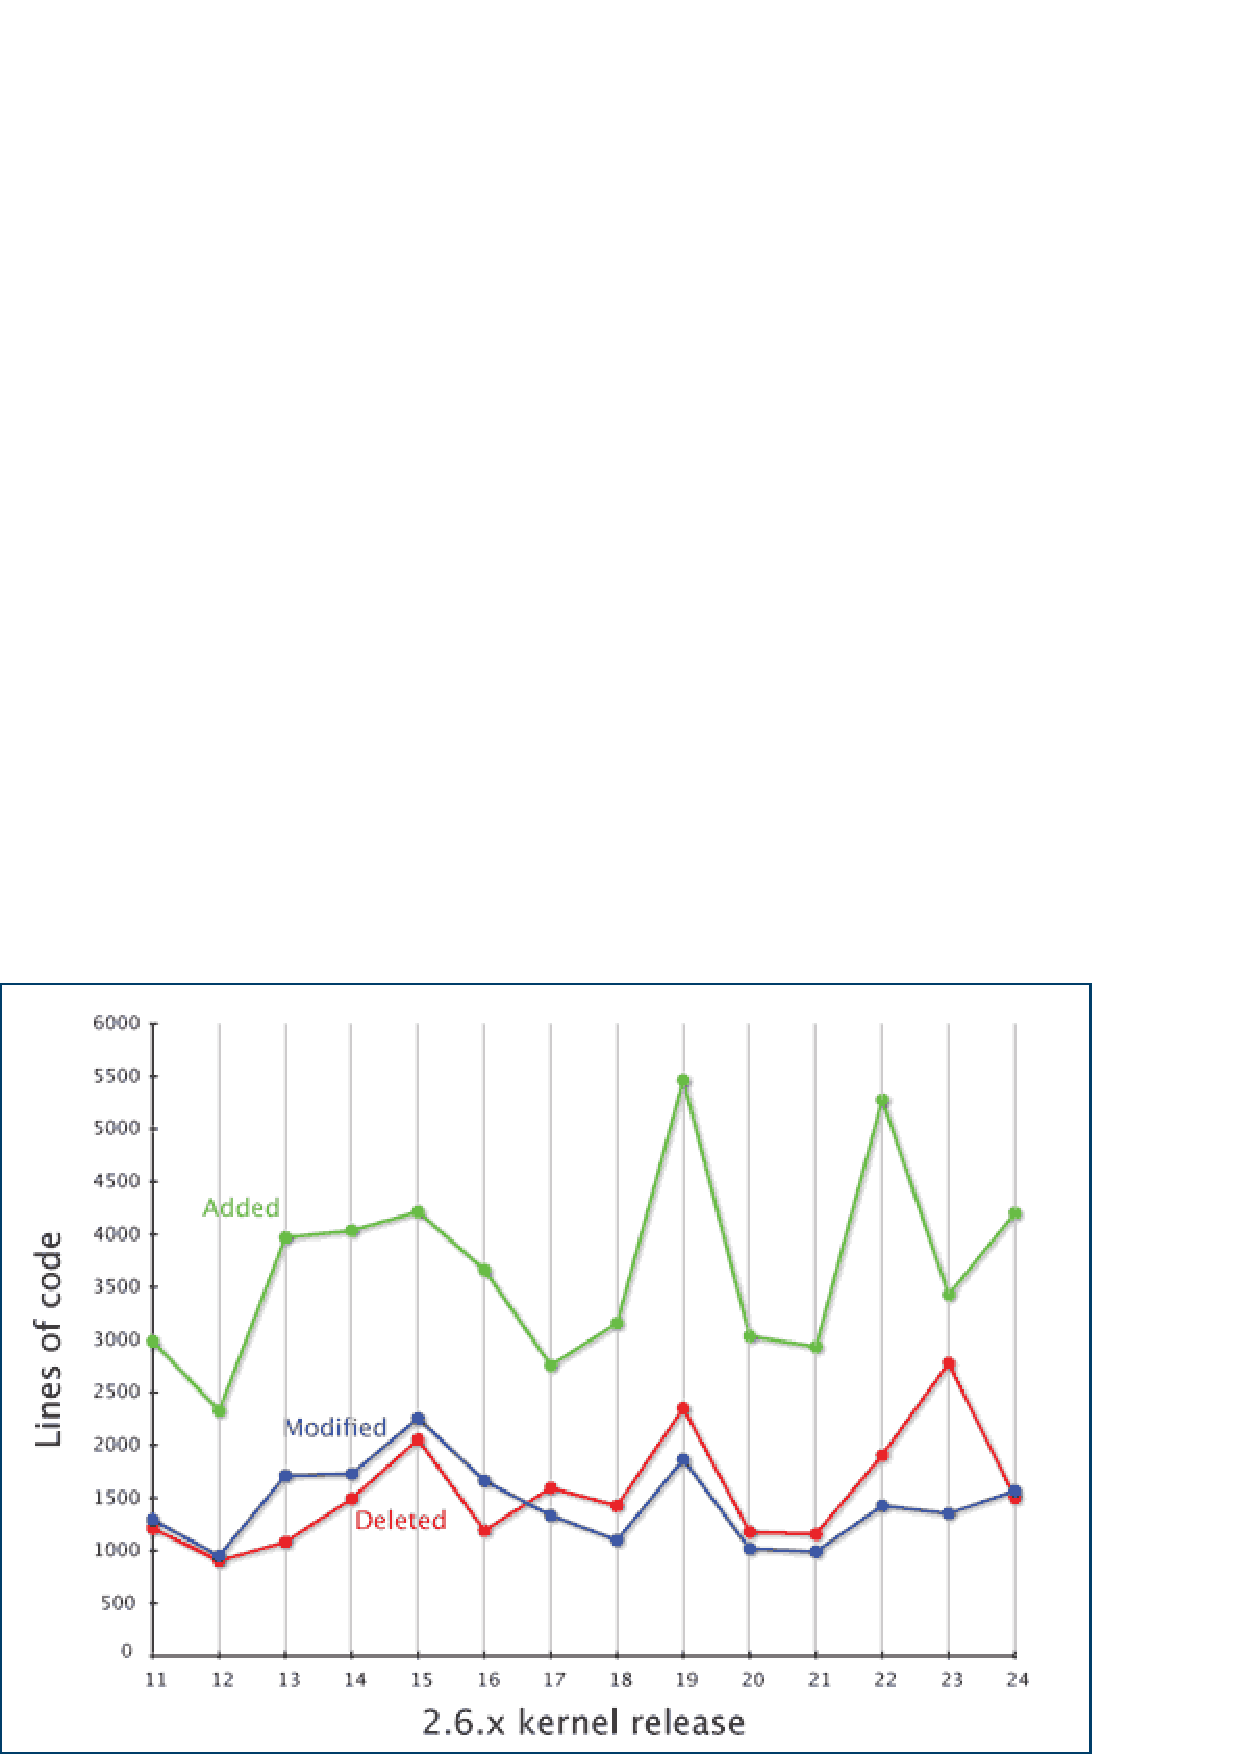
\includegraphics[width=9.5cm]{img/figure5-rateofchange.png}
\end{center}

Estas l\'{i}neas de c\'{o}digo sumaban en total en el 2008, nueve millones de l\'{i}neas de las cuales, aproxim\'{a}damente el 50-55\% representan drivers y el 5\% el \textit{core} del kernel. Se estima que cada a\~{n}o la cantidad de l\'{i}neas aumenta (crece) a velocidad constante (en un 10\%) y mantiene la correspondencia entre las proporciones de c\'{o}digo, es decir, aumenta por igual en todos sus componentes.

\begin{center}
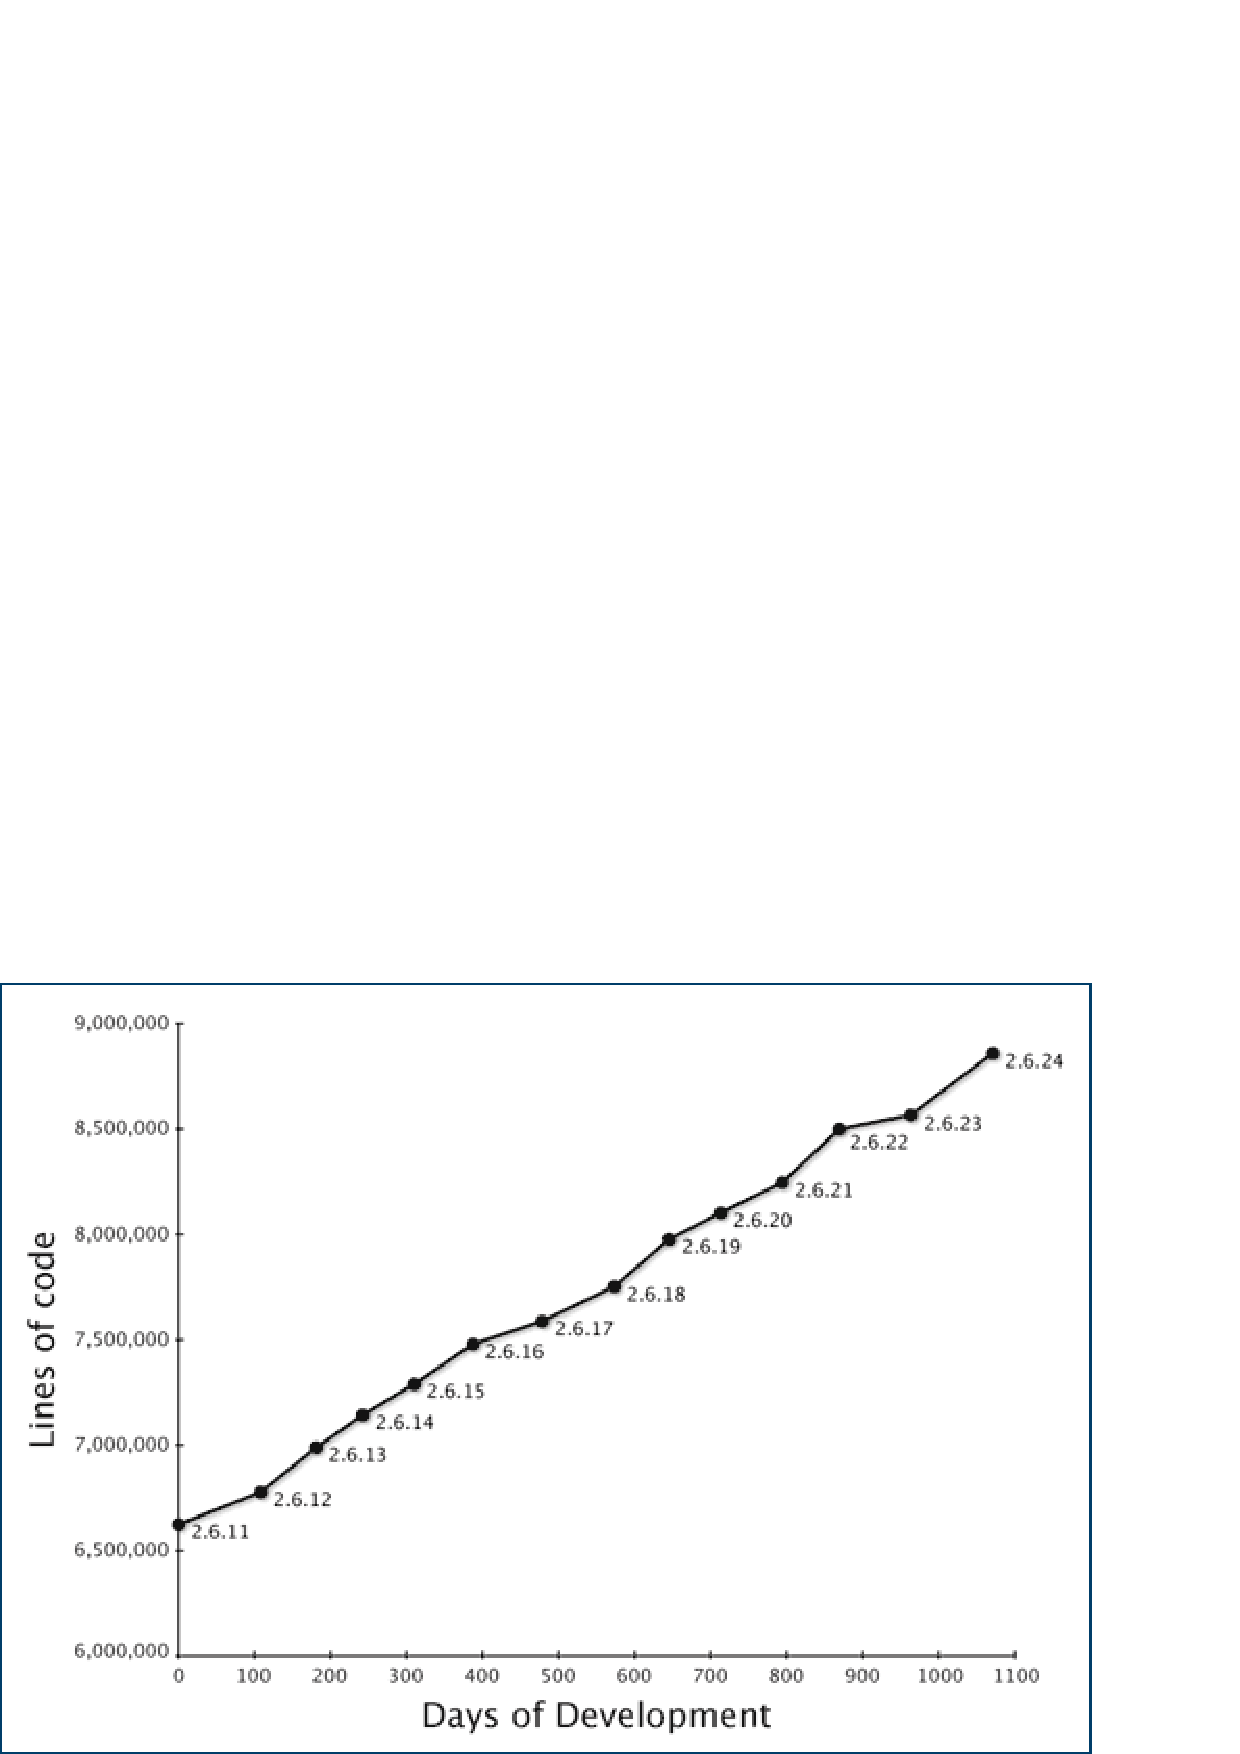
\includegraphics[width=9.5cm]{img/figure4-sizeperkernel.png}
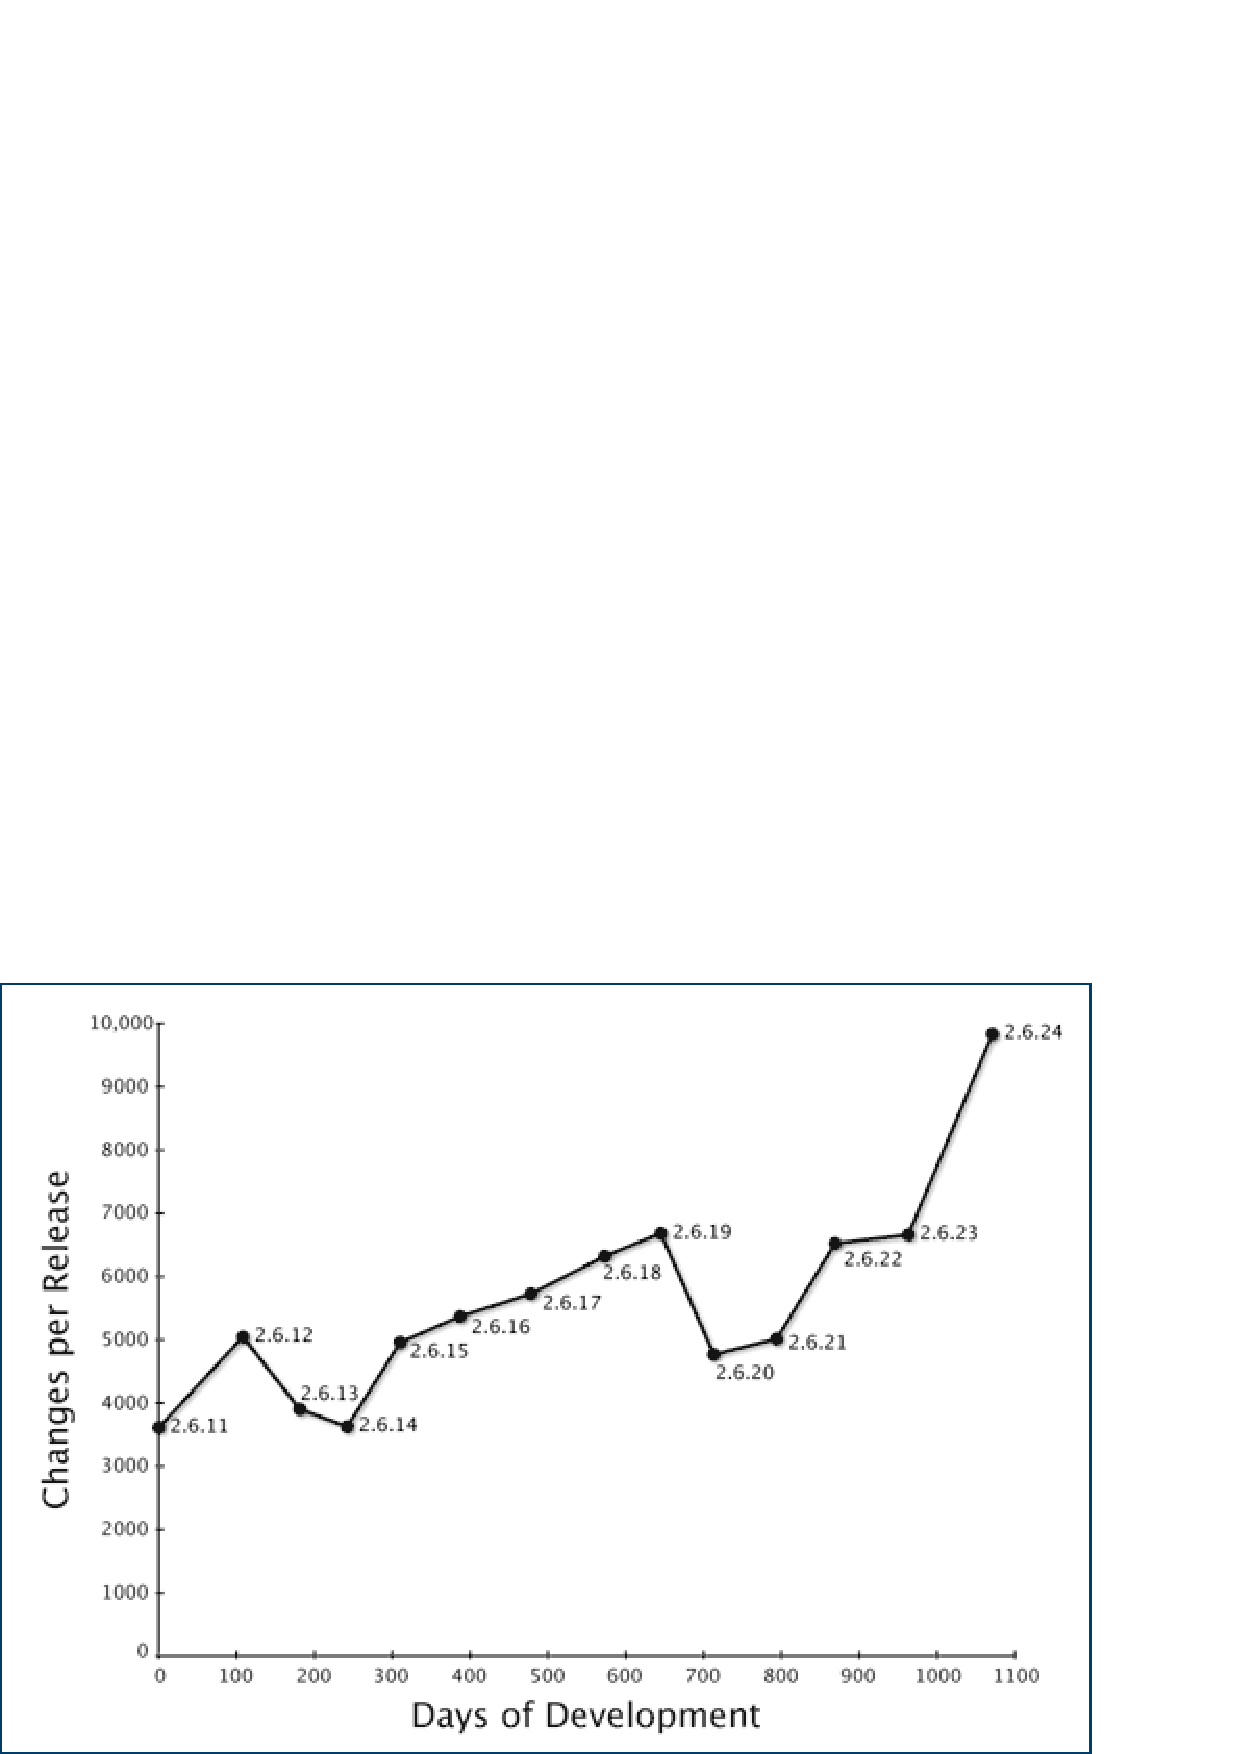
\includegraphics[width=9.5cm]{img/figure2-changesperkernel.png}
\end{center}

La modalidad de trabajo funciona de la siguiente manera:
\begin{enumerate}
	\item \textbf{Desarrolladores:} Hacen cambios, pueden arreglar un \textit{bug} o agregar un nuevo driver. Este desarrollador se lo manda al \textit{maintainer} (encargado) del archivo, cada archivo tiene uno.

	\item \textbf{Mantenedor de archivos:} Esta persona se encarga de revisar los cambios hechos por los desarrolladores y les da el \textit{visto bueno}, usualmente se le puede encontrar por ser la \'{u}ltima persona que toc\'{o} (con el comando \textit{touch}) el archivo, estos le mandan el archivo a los mantenedores del sub-sistema correspondiente. Exist\'{i}an en el 2008, aproximadamente 600 mantenedores de archivos.

	\item \textbf{Mantenedor de subsistema: } Esta persona es la \'{u}ltima en revisar el archivo. Existe un encargado por subsistema e.g. distribuci\'{o}n de \textit{ARM}, seguridad, redes, etc\'{e}tera.
	
	\item \textbf{Linux Next Tree}: Todas las noches, Stephen Rothwell h ace \textit{pulls} de los repositorios de cada subsistema en el repositorio \textit{Linux next}, les hace \textit{merge} y compruebe que todo compile y pase las pruebas.
	
	\item \textbf{Releases: } Cada dos semanas se hace un \textit{release candidate (RC)}, por ejemplo el 2.6.19.1.RC1, 2.6.19.1.RC2.. hasta que Linus Torvalds considere que es adecuado liberar la versi\'{o}n 2.6.19.1, aproxim\'{a}damente cada 2 $\frac{3}{4}$ meses.
\end{enumerate}

9.2 millones de lineas, desde el 2.6.0 (año X), cada año crece el 10\%. No todas las compus corren esos 9.2 millones... 2399 unique developers (la mitad solo commitearon 1 patch). Regla del 80-20 Por cantidad de patches mandados, el top 20 (personas), hicieron el 80% del trabajo eso en el 2.5 al 2.6. 

\subsection{Qui\'{e}n soporta el trabajo}

En el a\~{n}o 2008, las entidades en orden que m\'{a}s aportaban y daban soporte al desarrollo del kernel.
\begin{center}
\begin{tabular}{|l l l|}
  \hline
  \multicolumn{3}{|c|}{Soportadores del desarrollo de kernel} \\
  \hline
  1. & Amateurs (Aficionados) & 18.5\%\\
  2. & Red hat 				  & 11.5\%\\
  3. & IBM 					  & 7.5\%\\
  4. & Novell (Suse)            & 6.6\%\\
  5. & Individuales desconocidos & 5.5\%\\
  6. & Intel 				  & 4.1\%\\
  7. & Oracle 				  & 2.2\%\\
  8. & Consultants 			  & 2.2\%\\
  9. & Academa 				  & 1.5\%\\
  10. & Reneass Technology    & 1.5\%\\
  \hline
\end{tabular}
\end{center}


%Canonical tubo 6 changes en los ultimos 5 años  (lugar ~300).  75% del development del kernel es pagado (les importa).

%El userspace tratan de no cambiarlo! el API deberia de correr igual.

%Buscar Que es KVM (what is next le preguntaron) es bueno para el network latency
%USB 3.0



\section{Market share}

\subsection{Porcentaje del mercado}

\paragraph{Computadoras personales y portatiles.} En Junio de 2010, Linux tenía entre el 1\% \cite{NetMarketShare} y el 4\% \cite{W3C}de uso dentro de los sistemas operativos que navegaban en la web, estos normalmente los que son instalados en computadoras personales y portatiles.

\paragraph{\textit{Netbooks}.} Linux ocupaba el segundo lugar entre los sistemas operativos más usados en 2009, con un tercio (~34\%) del mercado, en ese año se estima que se habían vendido cerca de 35 millones de $netbooks$ \cite{ComputerWorld-LinusNetbookShare}. En 2007, cuando el mercado de las $netbooks$ iniciaba, Linux dominaba con 90\%. \cite{Gizmodo}

\paragraph{Servidores. } En el primer cuarto del 2010, la IDC (\texit{International Data Corporation} publicó que apróximadamente el 20\% del mercado pertenecía a Linux.  \cite{ComputerWorld-LinuxServers}, aunque otras otras fuentes con otros métodos de análisis, alegan que ese porcentaje es del 40\%, en el 2009. \cite{Netcraft}

\paragraph{Mainframes. } En 2010, totalmente dominado por el Sistema z de IBM \cite{OSNews}, aunque Red Hat alegaba el 18.4\% en 2007 y el 37\% en 2008. \cite{SearchDataCenter}

\paragraph{Supercomputadoras. } Dominado por Linux, en un 91\%, seguido por Unix (4.40\%) \cite{TOP500}.

\clearpage
\addcontentsline{toc}{chapter}{Bibliografía}
\begin{thebibliography}{99}
%referencias anteriores
\bibitem{sistosES}Silberschatz, A. et. al., \textit{Fundamentos de sistemas operativos.} 7a edición. McGRAW-HILL/INTERAMERICANA DE ESPAÑA,S.A.U. Bogotá, 2006. 
\bibitem{sistosEN}Silberschatz et al, \textit{Operating System Concepts.} John Wiley \& Sons, 7th edition, 2004. 
\bibitem{FHSWikipedia} Wikipedia Foundation, inc. \textit{Filesystem Hierarchy Standard}. \url{http://es.wikipedia.org/wiki/Filesystem_Hierarchy_Standard}. Fecha de consulta: 3 de Septiembre de 2010.
\bibitem{GregKorahHartman-GoogleTalk} Greg Korah Hartman on the Linux Kernel, Google Tech Talks, 5 de Junio del 2008, \url{http://www.youtube.com/watch?v=L2SED6sewRw}.
\url{http://es.wikipedia.org/wiki/Filesystem_Hierarchy_Standard}. Fecha de consulta: 29 de Agosto de 2010.
\bibitem{Linux-Capabilities-FAQ-0.2} Linux Capabilities FAQ 0.2, kernel.org, \url{http://www.kernel.org/pub/linux/libs/security/linux-privs/kernel-2.4/capfaq-0.2.txt}
\bibitem{clone2-manual} \textbf{clone(2)}, Linux man page, linux.die.net, \url{http://linux.die.net/man/2/clone}
\bibitem{MinixWikipedia}Wikpiedia Foundation, inc. \textit{Minix}. \url{http://es.wikipedia.org/wiki/Minix}. Fecha de consulta: 5 de Septiembre de 2010.  
\bibitem{ArchivoAlegsa}ALEGSA.com.ar. \textit{Definición de archivos de intercambio}. \url{http://www.alegsa.com.ar/Dic/archivo\%20de\%20intercambio.php}. Fecha de consulta: 5 de Septiembre de 2010.
\bibitem{TCPWikipedia}Wikpiedia Foundation, inc. \textit{Tamaño de ventana TCP, Transmission Control Protocol}. \url{http://es.wikipedia.org/wiki/Transmission_Control_Protocol#Tama.C3.B1o_de_ventana_TCP}. Fecha de consulta: 5 de Septiembre de 2010. 
\bibitem{SMPWikipedia}Wikipedia Foundation, inc. \textit{Symmetric Multi-processing}. \url{http://en.wikipedia.org/wiki/Symmetric_Multi-Processing}. Fecha de consulta: 5 de Septiembre de 2010. 
\bibitem{Linux2.6Kniggit}J. Pranevich. \textit{The Wonderful World of Linux 2.6}. \url{http://www.kniggit.net/wwol26.html}. Fecha de consulta: 5 de Septiembre de 2010.

%referencias de kmels
\bibitem{ext2fs-definition} Ext2fs Definition, linfo.org, \url{http://www.linfo.org/ext2.html}
\bibitem{NetMarketShare} \textit{Operating System Market Share},Net Applications, \url{http://marketshare.hitslink.com/operating-system-market-share.aspx?qprid=10}
\bibitem{W3C} \textit{OS Platform Statistics}, W3C, w3schools.com, \url{http://www.w3schools.com/browsers/browsers_os.asp}.
\bibitem{Gizmodo} \textit{Linux owns 1/3 of the netbook marketshare}, Agosto 2009, gizmodo.com, \url{http://gizmodo.com/5421500/linux-owns-13-of-the-netbook-marketshare}.
\bibitem{ComputerWorld-LinusNetbookShare} Eric Lai, \textit{Linux's share of netbooks surging, not sagging, says analyst}, ComputerWorld, computerworld.com, \url{http://www.computerworld.com/s/article/9140343/Linux_s_share_of_netbooks_surging_not_sagging_says_analyst}.
\bibitem{ComputerWorld-LinuxServers} \textit{Windows widens lead over Linux in the server market}, Junio 2010, computerworld.com, \url{http://blogs.computerworld.com/16263/windows_widens_lead_over_linux_in_the_server_market}
\bibitem{Netcraft} \textit{Operating System Share by Groups for Sites in All Locations}, Enero del 2009, Netcraft.com, \url{https://ssl.netcraft.com/ssl-sample-report//CMatch/osdv_all}
\bibitem{OSNews} David Adams, \textit{IBM Tightens Stranglehold Over Mainframe Market}, Julio 2008, OS News, osnews.com, \url{http://www.osnews.com/story/19958/IBM_Tightens_Stranglehold_Over_Mainframe_Market}
\bibitem{SearchDataCenter} Bill Claybrook, \textit{Red Hat bolsters Linux for mainframes, tries to catch Novell}, Search Data Center, techtarget.com, \url{http://searchdatacenter.techtarget.com/tip/0,289483,sid80_gci1366811,00.html}
\bibitem{TOP500} \textit{Operating system Family share for 06/2010}, Top500, top500.org, \url{http://top500.org/stats/list/35/osfam}


%referencias de hector
\bibitem{ZoneDMAThread} Calusic, Z. \textit{Tell me about ZONE\_DMA}. \url{http://mail.nl.linux.org/linux-mm/2000-07/msg00041.html}. Fecha de consulta: 6 de Septiembre de 2010. 
\bibitem{linuxDevices13}Rubini, A. y Corbet J. \textit{Chapter 13: nmap and DMA, Linux devices drivers} 2nd Edition. \url{http://www.xml.com/ldd/chapter/book/ch13.html}. Fecha de consulta: 7 de Septiembre de 2010.
\bibitem{LSBWikipedia}Wikipedia Foundation, inc. \textit{Linux Standard Base}. \url{http://en.wikipedia.org/wiki/Linux_Standard_Base#Criticism}. Fecha de consulta: 7 de Septiembre de 2010.
\bibitem{LinuxForWebsites}W3Techs Web Technology Surveys. \textit{Usage of Linux for websites}. \url{http://w3techs.com/technologies/details/os-linux/all/all}. Fecha de consulta: 7 de Septiembre de 2010. 
\bibitem{centosProblem}Perlow, J. \textit{CentOS: Getting their S#!t toghether is a top priority}. \url{http://www.zdnet.com/blog/perlow/centos-getting-their-st-together-is-a-top-priority/10790}. Fecha de consulta: 7 de Septiembre de 2010.
\bibitem{debianCost}Free Software Magazine. \textit{Impossible thing #1: Developing efficient, well engineered free software like Debian GNU/Linux}. \url{http://www.freesoftwaremagazine.com/books/mihrfc/impossible_thing_1_developing_efficient_free_software_like_gnu_debian}. Fecha de consulta: 7 de Septiembre de 2010.
\bibitem{LinusTorvaldsFedora}Morris, R. \textit{Linus Torvalds, Geek of the Week}. \url{http://www.simple-talk.com/opinion/geek-of-the-week/linus-torvalds,-geek-of-the-week/}. Fecha de consulta: 7 de Septiembre de 2010.
\bibitem{DistroWatch}DistroWatch.com. \url{http://distrowatch.com/index.php?dataspan=52}. Fecha de consulta 7 de Septiembre de 2010. 
\bibitem{OnlineIntruders}SecurityFocus. \textit{Online intruders hit Red Hat, Fedora project}. \url{http://www.securityfocus.com/news/11532}. Fecha de consulta: 7 de Septiembre de 2010.
\bibitem{macedonia}\textit{Every student in the republic of Macedonia to use Ubuntu-powered computer workstations}. \url{http://www.ubuntu.com/news/macedonia-school-computers}. Fecha de consulta: 7 de Septiembre de 2010.
\end{thebibliography}
\end{document}
